% =====================================================================================
%  Single-frame QWLSI wavefront reconstruction -- algorithm report
%  Source of truth: ..\recon_single_frame\qwlsi_single_frame.py  (C# port: src\Qwlsi.Core)
%  Build:  pdflatex QWLSI_Algorithm_Report.tex  (run twice for references)
% =====================================================================================
\documentclass[11pt,a4paper]{article}

\usepackage[margin=2.4cm]{geometry}
\usepackage[T1]{fontenc}
\usepackage{lmodern}
\usepackage{amsmath,amssymb,amsthm,bm,mathtools}
\usepackage{booktabs,array,tabularx}
\usepackage{graphicx}
\usepackage{xcolor}
\usepackage{tikz}
\usetikzlibrary{arrows.meta,positioning,shapes.geometric,calc,fit}
\usepackage{pgfplots}
\pgfplotsset{compat=1.16}
\usepackage{algorithm}
\usepackage{algpseudocode}
\usepackage[colorlinks=true,linkcolor=blue!50!black,citecolor=blue!50!black,urlcolor=blue!50!black]{hyperref}

\theoremstyle{definition}
\newtheorem{remark}{Remark}
\newtheorem{proposition}{Proposition}

% ---- notation shortcuts
\newcommand{\vr}{\bm{r}}
\newcommand{\vk}{\bm{k}}
\newcommand{\vs}{\bm{s}}
\newcommand{\vf}{\bm{f}}
\newcommand{\vu}{\bm{u}}
\newcommand{\ii}{\mathrm{i}}
\newcommand{\ee}{\mathrm{e}}
\newcommand{\dd}{\mathrm{d}}
\newcommand{\FT}{\mathcal{F}}
\newcommand{\IFT}{\mathcal{F}^{-1}}
\newcommand{\Dop}{\mathsf{D}}
\newcommand{\Vop}{\mathsf{V}}
\newcommand{\Aop}{\mathsf{A}}
\newcommand{\Pop}{\mathsf{P}}
\newcommand{\Real}{\operatorname{Re}}
\newcommand{\Imag}{\operatorname{Im}}
\newcommand{\wrap}{\operatorname{wrap}}
\newcommand{\code}[1]{\texttt{\small #1}}
\DeclareMathOperator{\clip}{clip}
\DeclareMathOperator{\argmin}{arg\,min}
\DeclareMathOperator{\sinc}{sinc}

\title{\textbf{Single-Frame Quadri-Wave Lateral Shearing Interferometry:\\
Theory and Algorithm of the QwlsiApp Wavefront Reconstruction}}
\author{Technical report accompanying \code{QwlsiApp} (C\#/.NET\,8) and its Python/MATLAB reference}
\date{Version 1.1.0 --- compiled \today}

\begin{document}
\maketitle

\begin{abstract}
\noindent
This report documents, with full derivations, the algorithm implemented in \code{QwlsiApp}: the reconstruction of
the optical path difference (OPD) $W(\vr)$ and of the complex optical field $U(\vr)=\sqrt{I}\,\ee^{\ii 2\pi W/\lambda}$ from
\emph{one} raw frame of a quadri-wave lateral shearing interferometer (QWLSI, a cross-grating placed a short distance
$d$ in front of a camera sensor). The method (i)~Fourier-demodulates the two orthogonal carrier lobes and the zero-order lobe of the
interferogram, (ii)~models each carrier lobe as a complex lateral-shear interferogram of the unknown wavefront,
(iii)~inverts the shear phases by a masked, weighted least-squares problem built on the \emph{exact} Fourier shear operator, solved by
Fourier-preconditioned conjugate gradients with model-based phase re-wrapping, and (iv)~assembles the intensity and the complex field.
Because a carrier-vector error is mathematically indistinguishable from defocus and astigmatism, a one-time carrier calibration from a flat frame is part
of the method; this is derived quantitatively. The report also covers the optional with-reference mode, the Zernike analysis (lens power, astigmatism, \dots),
the numerical implementation choices of the C\# port, and the validation evidence recorded in the project.
\end{abstract}

\tableofcontents
\newpage

% =====================================================================================
\section{Introduction and system overview}
% =====================================================================================
A quadri-wave lateral shearing interferometer \cite{Primot2000,Baffou2012} consists of a two-dimensional diffraction grating
(a ``cross grating'' of period $\Gamma$, designed so that the zeroth and even orders are suppressed) mounted at a short distance $d$ in front of a camera
sensor with pixel size $p$. The wave to be measured illuminates the grating, which splits it into four copies propagating at small angles. Over
the distance $d$ the copies separate laterally (``shear'') by a distance that is a small multiple of the pixel size; their overlap produces an interference pattern whose
modulation encodes the \emph{differences} of the wavefront between points a shear distance apart.

\paragraph{Why a single frame is enough.}
A classical phase-shifting interferometer needs several frames. Here the four-wave interference pattern is a carrier-modulated image:
in the spatial-frequency plane the information sits in separate \emph{lobes}, so one frame contains the zero-order (intensity) lobe, two
orthogonal shear-phase lobes, and conjugates. Spatial carrier-frequency demodulation
(the Fourier-transform method of Takeda \emph{et al.}~\cite{Takeda1982}) separates them. The Zernike conventions follow \cite{Noll1976,ANSI}.

\paragraph{What the app computes.}
Starting from one raw $4512\times4512$ frame the pipeline produces, on a decimated $1504\times1504$ output grid of pitch $3p=8.22\,\mu\mathrm{m}$:
the OPD $W$ (metres, piston/tilt removed), the pupil mask, the normalised intensity $I$, and the complex field $U$; plus Zernike-based statistics
(lens power in dioptres, astigmatism, RMS, PV).

\subsection{System parameters}
\begin{table}[h]
\centering
\caption{Default system parameters (editable in the app; \code{settings.json}).}
\begin{tabular}{llll}
\toprule
Symbol & Meaning & Value & Code name \\
\midrule
$\Gamma$ & cross-grating period & $16.44\ \mu$m & \code{Gamma} \\
$d$ & grating--sensor distance & $0.11$ mm & \code{d} \\
$p$ & sensor pixel pitch & $2.74\ \mu$m & \code{p} \\
$Z$ & relay zoom & $1$ & \code{Z} \\
$\lambda$ & wavelength & $650$ nm & \code{lam} \\
$N$ & sensor size (square) & $4512$ px & \code{N} \\
$D$ & decimation factor & $3$ & \code{DEC} \\
$M=N/D$ & output grid size & $1504$ & \code{M} \\
$R$ & spectral window radius & $695$ bins & \code{R} \\
$\vf_a,\vf_b$ & carrier vectors (calibrated) & see Sec.~\ref{sec:calib} & \code{calibration.json} \\
\bottomrule
\end{tabular}
\end{table}
The output pixel pitch is $D\,p/Z = 8.22\ \mu$m.

\subsection{Pipeline at a glance}
\begin{figure}[h]
\centering
\begin{tikzpicture}[
  node distance=5mm and 7mm,
  box/.style={draw,rounded corners=2pt,align=center,minimum height=9mm,minimum width=28mm,font=\small,fill=blue!6},
  out/.style={draw,rounded corners=2pt,align=center,minimum height=9mm,minimum width=28mm,font=\small,fill=green!10},
  arr/.style={-{Stealth[length=2.2mm]},thick}]
\node[box] (raw) {raw frame $i(\vr)$\\$4512^2$, float32};
\node[box,right=of raw] (fft) {mean removal\\real FFT $F[\vk]$};
\node[box,right=of fft] (demod) {window + decimate\\sub-bin ramp\\$\rightarrow A_0,A_a,A_b$};
\node[box,below=of demod] (mask) {mask $m$ from\\$\min(|A_a|,|A_b|)$};
\node[box,left=of mask] (int) {black level,\\normalise $\rightarrow I$};
\node[box,below=of mask] (solve) {masked LS + PCG\\re-wrap passes\\$\rightarrow W$};
\node[box,left=of solve] (calib) {carriers $\vf_a,\vf_b$\\(calibration or\\reference)};
\node[out,below=of solve] (field) {$U=\sqrt{I}\,\ee^{\ii2\pi W/\lambda}$};
\node[out,left=of field] (zern) {Zernike fit:\\power, astig., RMS, PV};
\draw[arr] (raw)--(fft); \draw[arr] (fft)--(demod);
\draw[arr] (demod)--(mask); \draw[arr] (mask)--(solve);
\draw[arr] (demod.west) -- ++(-0.25,0) |- (int.north) ;
\draw[arr] (calib)--(solve);
\draw[arr] (calib.north)--++(0,0.6)-|(demod.south west) ;
\draw[arr] (solve)--(field); \draw[arr] (solve.south west)--(zern.north east);
\draw[arr] (int.south)--++(0,-1.9)-|(field.north west);
\end{tikzpicture}
\caption{Data flow of one reconstruction. The carriers enter twice: they select the spectral windows, and they define the shear vectors of the inversion.}
\label{fig:pipeline}
\end{figure}

% =====================================================================================
\section{Physical model of the QWLSI interferogram}
\label{sec:physics}
% =====================================================================================

\subsection{Four-beam field behind the cross grating}
Let the wave under test at the grating plane be $E(\vr)=\sqrt{I(\vr)}\,\ee^{\ii\psi(\vr)}$ with phase
$\psi=2\pi W/\lambda$, where $W$ is the OPD. The cross grating transmits (to good approximation) four first-order beams. In the axes of the grating
their transverse spatial frequencies (cycles per metre) are
\begin{equation}
\vu_{1,2}=\pm\tfrac12\vu_a,\qquad \vu_{3,4}=\pm\tfrac12\vu_b,\qquad
\vu_a=\tfrac{2}{\Gamma}\hat{\bm e}_a,\ \ \vu_b=\tfrac{2}{\Gamma}\hat{\bm e}_b,\ \ \hat{\bm e}_a\perp\hat{\bm e}_b ,
\label{eq:beams}
\end{equation}
i.e.\ the orders $(\pm1,0)$ and $(0,\pm1)$ with $|\vu_{1}-\vu_2|=2/\Gamma$.
In the paraxial approximation, free propagation over $d$ of a beam carrying the transverse frequency $\vu$ displaces its envelope by
$\lambda d\,\vu$ (the ray direction is $\lambda\vu$) and adds a constant phase. Hence, for a smooth field,
\begin{equation}
E_k(\vr)\simeq t_k\,E(\vr-\bm\rho_k)\,\ee^{\ii 2\pi\vu_k\cdot\vr}\,\ee^{\ii\chi_k},\qquad
\bm\rho_k=\lambda d\,\vu_k ,
\label{eq:beamfield}
\end{equation}
with real amplitudes $t_k$ (equal for a symmetric grating) and constant phases $\chi_k$. The four envelopes sit at
$\pm\vs_a/2$ and $\pm\vs_b/2$, where the \emph{shear vectors} are
\begin{equation}
\vs_j=\lambda d\,\vu_j\quad(j=a,b),\qquad |\vs_j|=\frac{2\lambda d}{\Gamma}.
\label{eq:shear_phys}
\end{equation}
With the default values, $|\vs|=2(650\,\mathrm{nm})(0.11\,\mathrm{mm})/16.44\,\mu\mathrm{m}=8.70\,\mu\mathrm{m}=3.17$ pixels.
(In Baffou's notation, $\alpha=\Gamma/(4\pi d)$ is the inverse of the phase-gradient-to-fringe-shift gain; $|\vs|=2\lambda d/\Gamma$ is the same quantity.)

\subsection{Spectral content of the intensity}
The sensor records $i(\vr)=|\sum_{k=1}^4E_k|^2$ (plus offset and noise). Expanding,
\begin{equation}
i=\underbrace{\sum_k t_k^2 I(\vr-\bm\rho_k)}_{\text{zero order}}
+\sum_{k<l}2t_kt_l\sqrt{I(\vr-\bm\rho_k)I(\vr-\bm\rho_l)}\cos\!\Big(\psi(\vr-\bm\rho_k)-\psi(\vr-\bm\rho_l)+2\pi(\vu_k-\vu_l)\!\cdot\!\vr+\chi_k-\chi_l\Big).
\label{eq:intensity_expand}
\end{equation}
The pair $(1,2)$ has $\vu_1-\vu_2=\vu_a$ and $\bm\rho_{1,2}=\pm\vs_a/2$; the pair $(3,4)$ has $\vu_3-\vu_4=\vu_b$. The remaining four pairs give the
\emph{diagonal} frequencies $(\pm\vu_a\pm\vu_b)/2$. Therefore
\begin{equation}
i(\vr)=a_0(\vr)+\Big[a_a(\vr)\,\ee^{\ii2\pi\vu_a\cdot\vr}+a_b(\vr)\,\ee^{\ii2\pi\vu_b\cdot\vr}+\text{diagonal terms}+\text{c.c.}\Big],
\label{eq:lobes}
\end{equation}
with the complex lobe images
\begin{align}
a_0(\vr)&=\sum_k t_k^2\,I(\vr-\bm\rho_k)\ \approx\ 4t^2 I(\vr),\label{eq:a0}\\
a_j(\vr)&=t^2\,E\!\big(\vr-\tfrac{\vs_j}{2}\big)\,E^{*}\!\big(\vr+\tfrac{\vs_j}{2}\big)\,\ee^{\ii\Delta\chi_j},\qquad j\in\{a,b\}.\label{eq:aj}
\end{align}
Taking the argument of \eqref{eq:aj}:
\begin{equation}
\boxed{\ \arg a_j(\vr)=\sigma\,\frac{2\pi}{\lambda}\Big[W\!\big(\vr+\tfrac{\vs_j}{2}\big)-W\!\big(\vr-\tfrac{\vs_j}{2}\big)\Big]+\Delta\chi_j,\qquad \sigma=-1\ }
\label{eq:shearphase}
\end{equation}
This is exactly the model of the reference code (\code{solve\_opd}). The sign $\sigma=-1$ follows from the conventions used here
($\ee^{+\ii\psi}$ field phase, lobes at $+\vu_j$ taken as $\ee^{+\ii2\pi\vu_j\cdot\vr}$ components) and was confirmed against the
vendor map (a concave lens must give a bowl); it is not a free parameter. The constant $\Delta\chi_j$ is the unknown relative grating phase; it only
adds a constant to the differential phase, which corresponds to a \emph{tilt} of $W$ (see Sec.~\ref{sec:piston}).
The modulus is $|a_j|=t^2\sqrt{I(\vr-\vs_j/2)\,I(\vr+\vs_j/2)}$.

\begin{remark}[exactness of the central-difference model]
For this four-beam geometry the two beams that create carrier $a$ are displaced by exactly $\pm\vs_a/2$ about the same centre, so
\eqref{eq:shearphase} is a \emph{centred} difference with no approximation beyond the ideal four-beam model (\eqref{eq:beamfield}). Note that
the shear \emph{magnitude} is a fixed number of pixels ($\approx3.17$\,px) and not infinitesimal: the app never approximates the difference by a gradient.
\end{remark}

\subsection{The shear operator in the Fourier domain}
For $\vs$ in pixels and $\vk$ in cycles per pixel, the centred shear difference acts on a plane wave $\ee^{\ii2\pi\vk\cdot\vr}$ as
\begin{equation}
\ee^{\ii2\pi\vk\cdot(\vr+\vs/2)}-\ee^{\ii2\pi\vk\cdot(\vr-\vs/2)}=2\ii\sin(\pi\,\vk\cdot\vs)\,\ee^{\ii2\pi\vk\cdot\vr}.
\label{eq:Hsymbol}
\end{equation}
Hence the \emph{shear operator} is the Fourier multiplier
\begin{equation}
H_j(\vk)=2\ii\sin(\pi\,\vk\cdot\vs_j),\qquad \Dop_jW=\IFT\!\big[H_j\,\FT W\big].
\label{eq:H}
\end{equation}
This operator is \emph{exact for band-limited $W$}, i.e.\ it implements sub-pixel shifts by Fourier interpolation. The shear $\approx3.17$ px is $\approx1.06$ samples of the decimated grid
(spacing $D=3$ px), so a direct finite-difference stencil on the grid would be inaccurate; the Fourier form avoids that.
Three properties are used later.
\begin{enumerate}
\item $H_j(-\vk)=-H_j(\vk)$ and purely imaginary, so $\Dop_j$ maps real arrays to real arrays and its adjoint is $\Dop_j^{\mathsf T}=-\Dop_j$.
\item $H_j(\bm 0)=0$: constants are in the null space (piston is unobservable).
\item \textbf{No blind frequencies on the grid.} $H_j(\vk)=0$ requires $\vk\cdot\vs_j\in\mathbb Z$. The grid Nyquist is $|k_x|,|k_y|\le 1/(2D)=1/6$ cyc/px, and with the calibrated shears
$\vs_a\approx(2.664,-1.727)$, $\vs_b\approx(-1.727,-2.664)$\,px one has $|\vk\cdot\vs_j|\le\tfrac16(2.664+1.727)=0.732<1$. Hence $H_a$ and $H_b$ vanish simultaneously \emph{only} at $\vk=\bm0$.
(Derived here from the stated numbers.)
\end{enumerate}
For small $\vk\cdot\vs$, $H_j\approx2\pi\ii\,\vk\cdot\vs_j$, i.e.\ $\Dop_j\approx\vs_j\!\cdot\!\nabla$: the sensor measures the directional derivative of $W$ along two orthogonal directions, as every lateral shearing interferometer does.

\subsection{Sensitivity and a worked example}
For a spherical wavefront of power $P$ (dioptres), $W=Pr^2/2$ and $W(\vr+\vs/2)-W(\vr-\vs/2)=P\,\vr\cdot\vs$. The pupil radius implied by the mask
reported in the project (818\,720 pixels of $8.22\ \mu$m) is $R_p=\sqrt{818720\,(8.22\,\mu\mathrm m)^2/\pi}\approx4.2$ mm. For $P=1.5$ D at the pupil edge,
\[
|\arg a_j|_{\max}=\frac{2\pi}{\lambda}P\,R_p\,|\vs|=2\pi\,\frac{(1.5)(4.2\times10^{-3})(8.70\times10^{-6})}{650\times10^{-9}}\approx0.53\ \mathrm{rad}.
\]
So for the test lenses ($\pm0.7$ to $\pm1.5$ D) the differential phase never wraps; the re-wrapping passes of Sec.~\ref{sec:inversion} matter only for strongly aberrated wavefronts.
For a mode of spatial frequency $k$, $|H|\approx2\pi|\vs||\vk|$, so phase noise $\delta\varphi$ yields an OPD error $\propto\lambda\,\delta\varphi/(4\pi^2|\vs||\vk|)$: the noise gain
grows towards low spatial frequencies (as in every gradient-based sensor), which is why the low-order modes are the hardest to invert well and why the preconditioner of Sec.~\ref{sec:pcg} matters.

% =====================================================================================
\section{Spectral demodulation}
\label{sec:demod}
% =====================================================================================
\subsection{Discrete Fourier conventions}
Let $i[x,y]$ be the frame ($x$ = column, $y$ = row, $0\le x,y<N$). With the \emph{unnormalised} DFT
\begin{equation}
F[k_x,k_y]=\sum_{x,y}\big(i[x,y]-\mu\big)\,\ee^{-\ii2\pi(k_xx+k_yy)/N},\qquad \mu=\frac1{N^2}\sum i,
\label{eq:dft}
\end{equation}
a component $c\,\ee^{\ii2\pi\vf\cdot\vr}$ of the image with $\vf$ on the bin lattice $\vf=\bm k/N$ appears at $F[\bm k]=N^2c$. The mean is removed so that the
zero-order lobe is not dominated by the offset (it is added back later, Sec.~\ref{sec:intensity}). In the app the real-to-complex FFT stores only the half plane $k_x\ge0$; values elsewhere are
obtained from the Hermitian symmetry $F[-\bm k]=F[\bm k]^*$.

\subsection{Frequency-plane layout}
With $|\vf_a|=|\vf_b|=2p/\Gamma=1/3$ cyc/px, the carriers are at $N\vf\approx1504$ bins from the origin. With the calibrated values
$\vf_a=(0.27967,-0.18136)$ and $\vf_b=(-0.18137,-0.27974)$ cyc/px (angle $\theta=-0.5771$ rad, orthogonal to $10^{-5}$), the lobe centres in bins are
\[
\text{DC}:(0,0),\quad A:(1262,-818),\quad B:(-818,-1262),\quad \text{diagonals}:\ \pm\big(\tfrac{\vf_a+\vf_b}2\big)N=\pm(222,-1040),\ \ \pm\big(\tfrac{\vf_a-\vf_b}2\big)N=\pm(1040,222),
\]
plus the conjugates of $A,B$ (Figure~\ref{fig:spectrum}). The lobes used are the three solid circles; the four diagonal lobes are ignored by the pipeline
(they were used only in the rejected forward-model experiment, Sec.~\ref{sec:valid}).
\begin{figure}[h]
\centering
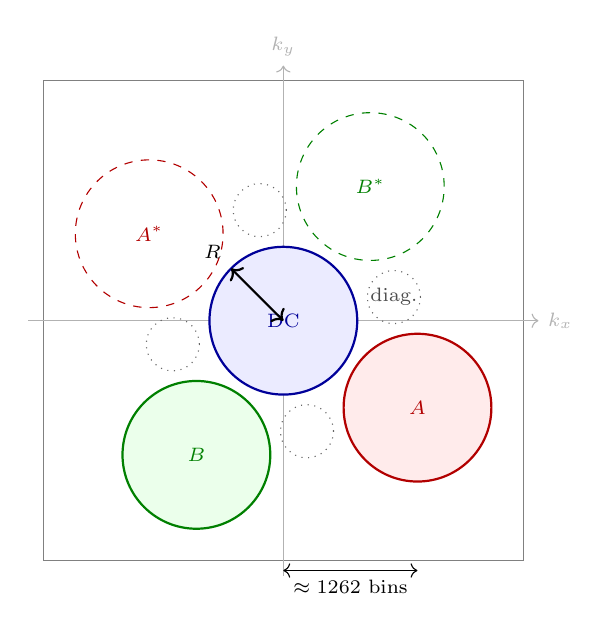
\begin{tikzpicture}[scale=1.35]
  % frame: Nyquist +-2256 bins -> units of 1000 bins
  \draw[gray] (-2.256,-2.256) rectangle (2.256,2.256);
  \draw[gray!60,->] (-2.4,0)--(2.4,0) node[right,font=\scriptsize]{$k_x$};
  \draw[gray!60,->] (0,-2.4)--(0,2.4) node[above,font=\scriptsize]{$k_y$};
  \draw[thick,blue!60!black,fill=blue!8] (0,0) circle (0.695) node[font=\scriptsize]{DC};
  \draw[thick,red!70!black,fill=red!8] (1.262,-0.818) circle (0.695) node[font=\scriptsize]{$A$};
  \draw[thick,green!50!black,fill=green!8] (-0.818,-1.262) circle (0.695) node[font=\scriptsize]{$B$};
  \draw[dashed,red!70!black] (-1.262,0.818) circle (0.695) node[font=\scriptsize]{$A^*$};
  \draw[dashed,green!50!black] (0.818,1.262) circle (0.695) node[font=\scriptsize]{$B^*$};
  \foreach \x/\y in {0.222/-1.040,-0.222/1.040,1.040/0.222,-1.040/-0.222}
     \draw[dotted,gray!80!black] (\x,\y) circle (0.25);
  \node[font=\scriptsize,gray!60!black] at (1.04,0.222) {diag.};
  \draw[<->] (0,-2.35)--(1.262,-2.35) node[midway,below,font=\scriptsize]{$\approx1262$ bins};
  \draw[<->,thick] (0,0)++(30:0) -- ++(135:0.695) node[font=\scriptsize,above left]{$R$};
\end{tikzpicture}
\caption{Spectral layout (axes in units of $10^3$ FFT bins of the $4512^2$ transform; Nyquist $=\pm2256$). Solid circles: the three windows
(radius $R=695$ bins) used for $A_0$ (zero order), $A_a$, $A_b$; dashed: conjugates; dotted: diagonal lobes (not used).}
\label{fig:spectrum}
\end{figure}

\paragraph{Window radius as a trade-off (derived here).}
The windows of $\mathrm{DC}$, $A$ and $B$ are mutually disjoint because $R=695<752=\tfrac12\cdot1504$ (half the distance from DC to $A$ or $B$)
and $695<\tfrac12\cdot2127$ for the $A$--$B$ distance. They do reach towards the diagonal lobes (centres $\approx1063$ bins from DC, $A$, $B$), so lobe leakage
is negligible only when the wavefront content is smooth enough that each lobe's own bandwidth is $\lesssim1063-695=368$ bins. The cut-off frequency $R/N=0.154$ cyc/px corresponds to
a smallest passed period of $6.5$ px ($\approx17.8\ \mu$m) at the sensor; in the output grid ($D=3$ px) this is below the Nyquist period of $6$ px, i.e.\ the window is
\emph{just inside} the output-grid Nyquist limit: $R=695<M/2=752$ bins, so no spectral wrap-around occurs when the window is copied into the $M\times M$ array.

\subsection{Windowed, decimated demodulation}
For a carrier $\vf$ let $\bm k_c=\mathrm{round}(N\vf)$ be the nearest integer bin. Define the circular, smooth-edged window on the $M\times M$ array
indexed by $\bm m\in\{-M/2,\dots,M/2-1\}^2$:
\begin{equation}
w(\bm m)=\tfrac12-\tfrac12\cos\!\big(\pi\,\tau(|\bm m|)\big),\qquad \tau(r)=\clip\!\Big(\frac{R-r}{\beta R},\,0,\,1\Big),\quad\beta=0.08 .
\label{eq:window}
\end{equation}
This is a flat top with a raised-cosine roll-off over the outer $8\,\%$ of the radius, from $r=0.92R=639$ to $r=R$ (Figure~\ref{fig:taper}); a smooth edge avoids Gibbs ringing in the demodulated image.
\begin{figure}[h]
\centering
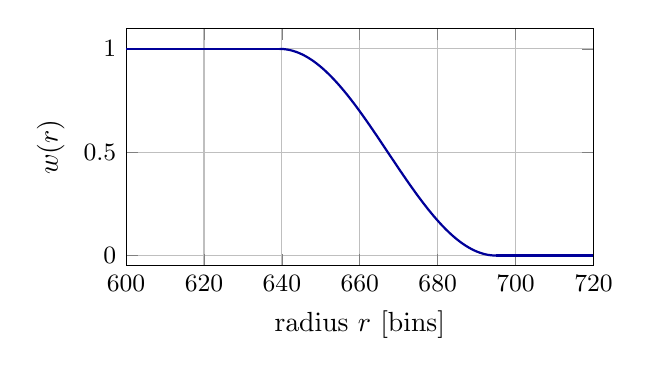
\begin{tikzpicture}
\begin{axis}[width=0.62\linewidth,height=4.6cm,xlabel={radius $r$ [bins]},ylabel={$w(r)$},xmin=600,xmax=720,ymin=-0.05,ymax=1.1,grid=both,
  tick label style={font=\small}]
\addplot[thick,blue!60!black,domain=600:639.4,samples=2]{1};
\addplot[thick,blue!60!black,domain=639.4:695,samples=80]{0.5-0.5*cos(180*((695-x)/55.6))};
\addplot[thick,blue!60!black,domain=695:720,samples=2]{0};
\end{axis}
\end{tikzpicture}
\caption{Radial profile of the spectral window \eqref{eq:window} ($R=695$, $\beta=0.08$).}
\label{fig:taper}
\end{figure}

The demodulated lobe is the inverse DFT of the windowed sub-spectrum $F[\bm k_c+\bm m]$ on the $M\times M$ grid:
\begin{equation}
z[\bm n]=\frac1{N^2}\sum_{\bm m}w(\bm m)\,F[\bm k_c+\bm m]\ \ee^{\ii2\pi\,\bm m\cdot\bm n/M},\qquad \bm n\in\{0,\dots,M-1\}^2 .
\label{eq:z}
\end{equation}
\textbf{Decimation is built in.} Evaluating the synthesis sum on $M$ points per axis with exponent $\ii2\pi mn/M=\ii2\pi m(Dn)/N$ is the same as sampling the full-resolution image at the pixels $x=Dn$;
since the window passes only $|\bm m|\le R<M/2$ bins the decimation is alias-free. The $1/N^2$ factor equals NumPy's $1/M^2$ inverse-FFT normalisation multiplied by $M^2/N^2$
(\code{(M*M)/(N*N)} in the code); with the forward normalisation \eqref{eq:dft} it returns the true complex amplitude of the lobe. An extra $D^2$ factor (applied in an early version) is wrong and distorted the intensity; the OPD is unaffected because only phases are used.

\subsection{Exact sub-bin carrier removal}
The true carrier is $\vf=\bm k_c/N+\bm\delta$ with $|\delta_x|,|\delta_y|\le\tfrac1{2N}$. By \eqref{eq:lobes}, $z[\bm n]$ is the lobe image $a(\vr)$ multiplied by the residual carrier $\ee^{\ii2\pi\bm\delta\cdot\vr}$
evaluated at $\vr=D\bm n$ (pixel units). The baseband lobe is obtained by multiplying with the conjugate ramp:
\begin{equation}
A_j[\bm n]=z[\bm n]\;\ee^{-\ii2\pi\,\bm\delta_j\cdot D\bm n},\qquad \bm\delta_j=\vf_j-\bm k_{c,j}/N .
\label{eq:ramp}
\end{equation}
This is the step that makes the method \emph{sub-bin-exact}: rounding the carrier to an integer bin would leave a residual phase ramp, which the inversion would misinterpret as a
wavefront with quadratic shape (Sec.~\ref{sec:calib}).

\subsection{Zero-order lobe, black level and intensity}
\label{sec:intensity}
The zero-order window ($\bm k_c=0$, no ramp) gives a real image $\Real z_0$ (the lobe is Hermitian-symmetric). The sum of the four shifted intensities \eqref{eq:a0} is
$I_0[\bm n]=\Real z_0[\bm n]+\mu$, with the mean restored. Outside the pupil $I_0$ contains only the camera offset. The \emph{black level} is estimated robustly as
\begin{equation}
\ell=\mathrm{P}_{10}(I_0),\qquad b=\operatorname{mean}\{I_0[\bm n]: I_0[\bm n]<1.5\,\ell+1\},
\end{equation}
and the normalised intensity is
\begin{equation}
I[\bm n]=\begin{cases}\max(I_0[\bm n]-b,0)\big/\mathrm{P}_{95}\big(\max(I_0-b,0)\big|_{m}\big)&\bm n\in\text{mask}\\ 0&\text{otherwise,}\end{cases}
\label{eq:I}
\end{equation}
where $\mathrm P_q$ is the $q$-th percentile and the 95th percentile is taken inside the mask only. A check recorded in the project: $|U|^2=I$ correlates $0.984$ with the smoothed raw frame.
The live transmittance view uses only this branch (one full FFT, the DC window, one small inverse FFT, black-level removal, normalisation) and requires neither carriers nor a calibration; with a reference
frame it shows $T=I/I_{\mathrm{ref}}$, with the denominator floored at $5\,\%$ of its 95th percentile.

% =====================================================================================
\section{Pupil mask}
\label{sec:mask}
% =====================================================================================
The inversion needs the set of pixels where both shear phases are trustworthy. From the two baseband lobes define $\alpha[\bm n]=\min(|A_a[\bm n]|,|A_b[\bm n]|)$ and
\begin{equation}
m_0=\{\alpha>0.15\,\mathrm P_{95}(\alpha)\},\quad m=\operatorname{erode}_{4}\!\Big(\operatorname{fill\_holes}\big(\operatorname{open}_{3}(m_0)\big)\Big).
\end{equation}
Morphological opening (3 iterations) removes isolated noise pixels, hole filling removes dark interior spots (e.g.\ dust), and a 4-pixel erosion ($\approx33\ \mu$m) discards the rim where
the finite-bandwidth window and the vanishing amplitude make the phase unreliable (the shear also pairs each point with a neighbour $\pm1.6$ px away, which must also be illuminated). The calibration uses stricter
parameters ($0.5$ instead of $0.15$, erosion $6$) so that only the clean centre of a flat beam enters the plane fit.

% =====================================================================================
\section{Wavefront inversion}
\label{sec:inversion}
% =====================================================================================
\subsection{Data, model and least-squares functional}
Let $c=\sigma\,2\pi/\lambda=-2\pi/\lambda$ and $\Vop=\operatorname{diag}(\mathbb 1_m)$ the mask as a diagonal operator on the $M\times M$ grid.
From each baseband lobe form the piston-free phase $\varphi_j=\arg\!\big(A_j\ee^{-\ii\arg\sum_{m}A_j}\big)$ (the complex-weighted mean phase is removed first, which is more robust than averaging wrapped phases). With the shear operator
\eqref{eq:H} (with $\vs_j$ in pixels and $\vk=\texttt{fftfreq}(M,d{=}D)$ in cycles/px) the unknown OPD minimises
\begin{equation}
J(W)=\sum_{j\in\{a,b\}}\big\|\Vop\,(c\,\Dop_jW-\varphi_j)\big\|^2+\varepsilon\|W\|^2,\qquad \varepsilon=10^{-9}.
\label{eq:J}
\end{equation}
The mask excludes unreliable pixels from the data term; the operator $\Dop_j$ itself acts on the full periodic grid (Fourier interpolation), so there is no zero-fill or periodic-boundary bias
inside the mask---a defect of simple Poisson/zero-fill integration, which under-estimates the amplitude by $\approx9\,\%$ at the pupil edge (project note, validated on a synthetic frame).
The tiny Tikhonov term fixes the piston null space.

\subsection{Normal equations and adjoint}
Setting $\nabla J=0$ and using $\Dop_j^{\mathsf T}=-\Dop_j$ (property 1 of Sec.~\ref{sec:physics}):
\begin{equation}
\underbrace{\Big(\sum_j\Dop_j^{\mathsf T}\Vop\Dop_j+\tfrac{\varepsilon}{c^2}\mathsf I\Big)}_{\Aop}\,W=\underbrace{\sum_j\Dop_j^{\mathsf T}\Vop\,\frac{\varphi_j}{c}}_{\bm b}.
\label{eq:normal}
\end{equation}
(The code adds $10^{-9}W$ to $\Aop W$ after dividing the data by $c$, which is the same up to the immaterial constant scaling of $\varepsilon$.)
$\Aop$ is symmetric positive definite on the complement of the constants, and each application costs two complex FFT pairs of size $M^2$ (one forward/inverse pair for $\Dop_j$ and one for $\Dop_j^{\mathsf T}$, each handling both $j$ at once; Sec.~\ref{sec:impl}), and each preconditioner application one real FFT pair.

\subsection{Why plain CG fails and what the preconditioner is}
\label{sec:pcg}
If $\Vop=\mathsf I$ (full mask) the operator is diagonal in Fourier space with symbol
\begin{equation}
S(\vk)=|H_a(\vk)|^2+|H_b(\vk)|^2=4\big[\sin^2(\pi\vk\cdot\vs_a)+\sin^2(\pi\vk\cdot\vs_b)\big],
\end{equation}
and for small $\vk$ with orthogonal shears of equal length $S\approx4\pi^2|\vs|^2|\vk|^2$ -- a (negative) Laplacian symbol. The condition number of such an operator on an $M\times M$ grid scales like $M^2$, and the
smooth, low-order modes (defocus-like) have the smallest eigenvalues. Unpreconditioned CG converges extremely slowly on those modes; this was observed in practice (project note: ``plain CG does not converge on defocus-like modes'').

The preconditioner is the (regularised) Fourier-space inverse of the \emph{unmasked} operator:
\begin{equation}
\Pop=\IFT\,\mathrm{diag}\big(P(\vk)\big)\,\FT,\qquad
P(\vk)=\begin{cases}\dfrac1{S(\vk)+10^{-6}S_{\max}+10^{-12}},&\vk\ne\bm0\\[2mm]0,&\vk=\bm 0.\end{cases}
\label{eq:precond}
\end{equation}
The $10^{-6}S_{\max}$ term bounds the gain at the weakest-sensitivity frequencies; $P(\bm0)=0$ keeps piston out.
Write the masked operator as $\Aop=\sum_j\Dop_j^{\mathsf T}\Dop_j-\mathsf E$, with $\mathsf E=\sum_j\Dop_j^{\mathsf T}(\mathsf I-\Vop)\Dop_j\succeq0$ supported on the \emph{excluded} region. Then
\[
\Pop\Aop\;\approx\;\mathsf I-\Pop\mathsf E ,
\]
so the preconditioned operator is the identity plus a perturbation that is only active on modes that matter in the masked-out area. Its eigenvalues cluster at $1$, which gives fast CG convergence
(a heuristic argument, borne out by the validated results with $60$ iterations). For the same reason the initial guess
\begin{equation}
W^{(0)}=\Pop\,\bm b
\end{equation}
(the direct Fourier-domain, zero-filled least-squares integration) already captures the low-order modes; CG then corrects the mask-edge errors. The project notes that \emph{both} the preconditioner and the initial guess are required.

\subsection{Preconditioned conjugate gradients}
Algorithm~\ref{alg:pcg} is the standard PCG recursion; the stopping tolerance is $\|r\|<\mathrm{rtol}\,\|\bm b\|$ with $\mathrm{rtol}=10^{-7}$ and at most $60$ iterations per pass.
\begin{algorithm}[h]
\caption{PCG for $\Aop W=\bm b$ (one pass)}
\label{alg:pcg}
\begin{algorithmic}[1]
\State $W\gets W^{(0)}$;\quad $r\gets\bm b-\Aop W$
\For{$t=0,1,\dots,t_{\max}-1$}
  \If{$\|r\|<10^{-7}\|\bm b\|$} \textbf{break} \EndIf
  \State $z\gets\Pop r$;\quad $\rho\gets\langle r,z\rangle$
  \State $q\gets z$ if $t=0$, else $q\gets z+(\rho/\rho_{\text{prev}})\,q$
  \State $\alpha\gets\rho/\langle q,\Aop q\rangle$
  \State $W\gets W+\alpha q$;\quad $r\gets r-\alpha\Aop q$;\quad $\rho_{\text{prev}}\gets\rho$
\EndFor
\State \Return $W$
\end{algorithmic}
\end{algorithm}

\subsection{Phase wrapping and the re-wrap passes}
The measured $\varphi_j$ are wrapped to $(-\pi,\pi]$. Where the true differential phase exceeds $\pi$ the wrapped data are inconsistent with a smooth $W$ and bias the LS solution.
The remedy is a model-based re-wrapping iteration. After pass $\ell$ with solution $W_\ell$ and prediction $\hat\varphi_j=c\,\Dop_jW_\ell$:
\begin{equation}
\varphi_j^{(\ell+1)}=\hat\varphi_j+\wrap\!\Big(\arg A_j-\hat\varphi_j\Big)=\hat\varphi_j+\arg\!\big(A_j\,\ee^{-\ii\hat\varphi_j}\big),
\qquad \varphi_j^{(\ell+1)}\leftarrow\varphi_j^{(\ell+1)}-\overline{\varphi_j^{(\ell+1)}}\big|_m .
\label{eq:rewrap}
\end{equation}
The residual between data and model is wrapped to its principal value and added back to the model, so the data are unwrapped \emph{to the nearest $2\pi$ multiple around the current estimate}.
This is correct whenever the current estimate is within $\pm\pi$ of the truth for each pixel, and each pass improves the estimate. The overall loop is $1+2=3$ passes (initial solve and two re-wraps),
each of up to $60$ CG iterations from a freshly preconditioned initial guess. The subtracted mean in \eqref{eq:rewrap} removes the constant differential phase, which corresponds to a tilt of $W$ (Sec.~\ref{sec:piston}).
At the end the app reports the masked RMS residuals $\big\|\Vop(\hat\varphi_j-\varphi_j)\big\|_{\mathrm{rms}}$ (radians) per carrier, next to the data RMS, as a quality measure.

\begin{algorithm}[h]
\caption{Reconstruction of one frame (\code{reconstruct})}
\label{alg:recon}
\begin{algorithmic}[1]
\Require frame $i$, carriers $\vf_a,\vf_b$ (calibration or reference), parameters $\lambda,d,p,D,R$
\State $\mu\gets\operatorname{mean}(i)$;\quad $F\gets\mathrm{rFFT}(i-\mu)$
\State $A_a\gets\textsc{Baseband}(F,\vf_a)$;\ $A_b\gets\textsc{Baseband}(F,\vf_b)$;\ $I_0\gets\Real\,\textsc{Window}(F,\bm0)+\mu$
\State $m\gets\textsc{MakeMask}(A_a,A_b)$
\If{reference given} \State $A_j\gets A_j\,\overline{A_j^{\mathrm{ref}}}$ for $j=a,b$ \EndIf
\State $\varphi_j\gets\arg\big(A_j\,\ee^{-\ii\arg\sum_mA_j}\big)$;\quad build $H_j$, $P$ from $\vs_j=\lambda d\vf_j/p^2$
\For{$\ell=0,1,2$}
  \State $\bm b\gets\sum_j\Dop_j^{\mathsf T}\Vop\varphi_j/c$;\quad $W\gets\textsc{PCG}(\Aop,\bm b,\ x_0=\Pop\bm b)$
  \If{$\ell<2$} \State re-wrap $\varphi_j$ via \eqref{eq:rewrap} \EndIf
\EndFor
\State $W\gets W-\overline{W}|_m$ on $m$, $\mathrm{NaN}$ outside;\quad $I\gets$ \eqref{eq:I};\quad $U\gets\sqrt I\,\ee^{\ii2\pi W/\lambda}\,m$
\State statistics from the Zernike fit (Sec.~\ref{sec:zern})
\end{algorithmic}
\end{algorithm}

% =====================================================================================
\section{Piston, tilt, the complex field and the reference mode}
\label{sec:piston}
% =====================================================================================
\paragraph{Piston and tilt.}
Piston lies in the null space of the shear operator (property 2) and is set by subtracting the masked mean of $W$. A constant added to the differential phase
(the unknown grating phase $\Delta\chi_j$ in \eqref{eq:shearphase}) corresponds to $W\to W+\bm g\cdot\vr$ with $\vs_j\cdot\bm g=\text{const}$, a tilt; since $\Delta\chi_j$ is not
known from a single frame, the \emph{absolute tilt is not measurable} and the delivered OPD is tilt-free (the differential phases are forced to zero mean in the re-wrapped passes, and the Zernike tilt terms can additionally be removed in the viewer).

\paragraph{Complex field.}
\begin{equation}
U(\vr)=\sqrt{I(\vr)}\,\exp\!\Big(\ii\frac{2\pi}{\lambda}W(\vr)\Big)\,m(\vr),
\end{equation}
stored as complex64. It is the field at the sensor plane; the grating plane lies $d=0.11$ mm earlier, which is negligible for smooth fields (the propagation over $d$ is ignored in \eqref{eq:beamfield}).

\paragraph{Reference (with-reference) mode.}
The OPD obtained without a reference contains the static system wavefront (beam and grating aberrations, $\approx0.3$--$0.4\ \mu$m RMS). If a flat/reference frame is available its lobes $A_j^{\mathrm{ref}}$ are demodulated with the
same windows and the sample lobes are replaced by
\begin{equation}
A_j\;\longrightarrow\;A_j\,\overline{A_j^{\mathrm{ref}}},\qquad
\arg\big(A_j\overline{A_j^{\mathrm{ref}}}\big)=\sigma\tfrac{2\pi}{\lambda}\,\Dop_j\big(W-W^{\mathrm{ref}}\big)+\text{const}.
\end{equation}
The static aberration cancels by linearity of $\Dop_j$ and the solver then returns the \emph{sample-only} OPD $W-W^{\mathrm{ref}}$. The carriers are taken from the reference frame itself, so no separate calibration is needed;
the amplitude weighting by $|A_j^{\mathrm{ref}}|$ is irrelevant to the solver (only the argument is used). The mask is computed from the lobes \emph{before} the multiplication; the intensity is unchanged.
Equivalent to first order: subtracting a stored reference OPD from the single-frame OPD (agreement of the two routes $\approx5$ nm, project note).

% =====================================================================================
\section{Carrier calibration}
\label{sec:calib}
% =====================================================================================
\subsection{A carrier error is a quadratic wavefront}
\label{sec:degen}
Suppose the carrier used in \eqref{eq:ramp} is $\vf_j+\bm\epsilon_j$ instead of the true $\vf_j$. The baseband lobe acquires the extra phase ramp $2\pi\bm\epsilon_j\cdot\vr$ ($\vr$ in pixels).
In the inversion this ramp must be explained by the shear model: $\sigma\frac{2\pi}\lambda\,\vs_j\!\cdot\!\nabla W=2\pi\bm\epsilon_j\cdot\vr$ (small-shear limit), i.e.\ $\nabla W$ is linear in $\vr$, and $W$ is \emph{quadratic}:
a defocus/astigmatism term. For orthogonal shears of length $s$ (pixels) the Laplacian of the spurious wavefront is (in physical units, $\vf$ in cycles/px, $p$ pixel pitch)
\begin{equation}
\nabla^2W_{\mathrm{err}}=\frac{\epsilon_{a\parallel}+\epsilon_{b\parallel}}{d\,|\vf|},\qquad
\Delta P=\tfrac12\nabla^2W_{\mathrm{err}}=\frac{\epsilon_{a\parallel}+\epsilon_{b\parallel}}{2\,d\,|\vf|}\ \ [\text{D}],
\label{eq:caldefocus}
\end{equation}
where $\epsilon_{j\parallel}$ is the component of $\bm\epsilon_j$ along $\vf_j$ and the sign follows $\sigma$ (derived here; the factor $\lambda$ cancels because $s_{\mathrm{px}}=\lambda d|\vf|/p^2$).
Numerically $2d|\vf|=2(0.11\,\mathrm{mm})/3=7.3\times10^{-5}$ m, so \emph{one FFT bin} of carrier error ($1/4512=2.2\times10^{-4}$ cyc/px) on one axis gives $\approx3$ D, and $10^{-5}$ cyc/px on both axes $\approx0.27$ D.
This matches the project's observation that the nominal carriers, which are off by $0.24$ bin on the second axis in this system, give a $3.7\ \mu$m RMS wavefront error and $\sim\pm1$ D power error, while everything of higher order is fine.
The perpendicular components of $\bm\epsilon_j$ produce the non-axisymmetric part (astigmatism and the non-integrable, curl part which least squares projects out).

\textbf{Consequence.} Carrier error \emph{cannot} be detected from the data of a single sample frame. The carriers are therefore established once, from a frame where the true wavefront is known to be flat (a collimated beam):
then any remaining phase ramp in the lobes is purely a carrier error and can be measured.

\subsection{Nominal carriers and DFT peak search}
Nominal values: $|\vf|=f_0=2p/\Gamma=0.3333$ cyc/px, $\vf_b$ equal to $\vf_a$ rotated by $-90^\circ$. The algorithm (\code{nominal\_carriers}) is:
\begin{enumerate}
\item Find the strongest bin of $|F|$ in the annulus $\big||\vk|/N-f_0\big|<20/N$, restricted to $k_x>0$.
\item Refine by maximising the \emph{continuous-frequency} DFT magnitude
\begin{equation}
\mathcal M(\vf)=\Big|\sum_{x,y}\big(i[x,y]-\mu\big)\,\ee^{-\ii2\pi(f_xx+f_yy)}\Big|
\end{equation}
over $\vf\in\mathbb R^2$ with the Nelder--Mead simplex method (tolerances $x_{\mathrm{tol}}=10^{-9}$, $f_{\mathrm{tol}}=10^{-3}$), evaluated separably in double precision. This is valid for an almost flat wave and biased by strong curvature.
\item Repeat for $\vf_b$, starting at $\vf_a$ rotated by $-90^\circ$; form the orientation $\theta=\arg(\ee^{\ii\theta_a}+\ee^{\ii\theta_b'})$ with $\theta_b'=\theta_b+\pi/2$, and set
$\vf_a=f_0(\cos\theta,\sin\theta)$, $\vf_b=f_0(\cos(\theta-\pi/2),\sin(\theta-\pi/2))$ (orthogonality and equal magnitude enforced).
\end{enumerate}

\subsection{Refinement from a flat frame}
Starting from the nominal $\vf$, repeat three times (\code{calibrate\_from\_flat}):
\begin{enumerate}
\item demodulate the lobe $A=\textsc{Baseband}(F,\vf)$, mask $m=\operatorname{erode}_6(\operatorname{fill}(\operatorname{open}_3(|A|>0.5\,\mathrm P_{95}|A|)))$, remove the piston $\arg\sum_m A$;
\item fit the phase plane by linear least squares, $\varphi(\vr)\approx g_xx+g_yy+g_0$ over $m$ ($\vr$ in sensor pixels);
\item update $\vf\leftarrow\vf+\bm g/2\pi$.
\end{enumerate}
The update follows from $A=a\,\ee^{\ii2\pi(\vf_{\mathrm{true}}-\vf)\cdot\vr}$ with $a$ of constant phase for a flat wave. Iteration is needed because the window is centred on the nearest integer bin of the \emph{current} estimate. The result is stored in \code{calibration.json} (schema shared by the
Python, MATLAB and C\# versions): $\vf_a=(0.2796747,-0.1813622)$, $\vf_b=(-0.1813663,-0.2797383)$ cyc/px for the delivered system. The app reports the size of the last update and the plane-fit residual per carrier as convergence diagnostics; the round-trip acceptance criterion is $10^{-5}$ cyc/px
(Python/Octave agree to $10^{-8}$). A frame averaged over several flats may be used to reduce noise.

\subsection{Other wavelengths and sensitivity to $d$}
The shear vector $\vs_j=\lambda d\vf_j/p^2$ and the factor $c=-2\pi/\lambda$ both contain $\lambda$; for small shear $W\approx c^{-1}\Dop^{-1}\varphi\propto\lambda\cdot(\lambda d)^{-1}$, so the OPD in metres is, to first order, independent of $\lambda$ but \emph{inversely proportional to the grating--sensor distance $d$}: a $1\,\%$ error in $d$ scales every OPD by $1\,\%$ (derived here from \eqref{eq:J}). The wavelength still enters the finite-shear model $\sin(\pi\vk\cdot\vs)$, the complex-field phase $2\pi W/\lambda$ and the physical carrier positions, so for another wavelength the app requires $\lambda$ to be set, a re-check of the carriers on a flat frame (which should read $0.00$ D), and a new flat-based system wavefront.

% =====================================================================================
\section{Zernike analysis and lens power}
\label{sec:zern}
% =====================================================================================
\subsection{Basis}
The app uses the OSA/ANSI (Z80.28) Zernike polynomials, radial orders $n=0,\dots,10$ (66 terms), single index $j=\big(n(n+2)+m\big)/2$, each normalised to unit RMS over the unit disk:
\begin{align}
Z_n^m(\rho,\theta)&=N_n^m\,R_n^{|m|}(\rho)\times\begin{cases}\cos(m\theta)&m\ge0\\ \sin(|m|\theta)&m<0\end{cases},\qquad N_n^m=\sqrt{(2-\delta_{m0})(n+1)},\\
R_n^{|m|}(\rho)&=\sum_{s=0}^{(n-|m|)/2}\frac{(-1)^s\,(n-s)!}{s!\,\big(\tfrac{n+|m|}2-s\big)!\,\big(\tfrac{n-|m|}2-s\big)!}\,\rho^{\,n-2s}.
\end{align}
Examples: $Z_1^{-1}=2\rho\sin\theta$, $Z_1^{1}=2\rho\cos\theta$, $Z_2^{-2}=\sqrt6\rho^2\sin2\theta$, $Z_2^0=\sqrt3(2\rho^2-1)$ (defocus), $Z_4^0=\sqrt5(6\rho^4-6\rho^2+1)$ (spherical).
The reference script fits to $n_{\max}=6$; the app fits all $66$ terms jointly.

\subsection{Fit and orientation}
The pupil circle is derived from the mask: centre = centroid of $m$, radius $r_p=\sqrt{|m|/\pi}$ pixels (physical $R_m=r_p\cdot Dp/Z$). With $\rho=|\vr-\vr_c|/r_p$ the coefficients $c_i$ minimise
\begin{equation}
\sum_{\vr\in m,\ \rho\le1}\Big(W(\vr)-\sum_ic_iZ_i(\rho,\theta)\Big)^2 .
\end{equation}
Subtraction of selected terms is evaluated at every valid mask pixel (also $\rho>1$) and is non-destructive. $\theta$ is measured counter-clockwise from $+x$ with $y$ up in the app (the Python reference uses $y$ down; the app's \code{FlipY} setting reproduces it); the orientation-independent quantities (power, astigmatism magnitude, coma magnitude, spherical) do not change.

\subsection{Reported quantities}
For defocus coefficient $c_2^0$ the quadratic part of $W$ is $2\sqrt3\,c_2^0\,r^2/R_m^2$, to be compared with $Pr^2/2$ for a sphere of power $P$, hence
\begin{equation}
P=\frac{4\sqrt3\,c_2^{0}}{R_m^{2}}\ \ [\mathrm D]\quad(+=\text{concave/bowl}),\qquad
A_{\mathrm{ast}}=\sqrt{(c_2^{2})^2+(c_2^{-2})^2},\qquad
A_{\mathrm{coma}}=\sqrt{(c_3^{1})^2+(c_3^{-1})^2}.
\end{equation}
The astigmatism power-vector components are $2\sqrt6\,c/R_m^2$. RMS is the standard deviation of $W$ over $m\cap\{\rho\le1\}$, and PV its range. Examples: concave\_1: $+0.711$ D (order-6 report), $+0.7109$ D (order-10 joint fit).

% =====================================================================================
\section{Numerical implementation (C\# port)}
\label{sec:impl}
% =====================================================================================
The port (\code{Qwlsi.Core}) follows the Python functions one-to-one (Appendix~\ref{app:map}); the changes are numerical, not algorithmic.

\paragraph{FFTs and precision.}
All hot-path arrays are \code{float32} and pre-allocated; FFTs use Intel MKL (or FFTW) through P/Invoke. The $4512^2$ transform is real-to-complex (half spectrum); the lobe windows read the half spectrum via Hermitian symmetry.
The solver uses $1504^2$ complex and real transforms in parallel across cores.

\paragraph{Packing two real transforms in one complex FFT.}
Both $\Dop_0W$ and $\Dop_1W$ are real. With $G=H_0+\ii H_1$,
$\IFT[G\,\FT W]=\Dop_0W+\ii\,\Dop_1W$, so one complex forward/inverse pair gives both shears. For the adjoint, pack $r_0+\ii r_1$ and use
$T=\FT(r_0+\ii r_1)=R_0+\ii R_1$ with $R_0=\tfrac12(T+\tilde T)$, $R_1=\tfrac1{2\ii}(T-\tilde T)$, $\tilde T(\vk)=\overline{T(-\vk)}$:
\begin{equation}
H_0R_0+H_1R_1=\tfrac12(H_0-\ii H_1)\,T+\tfrac12(H_0+\ii H_1)\,\tilde T,
\end{equation}
and $\Dop^{\mathsf T}\text{-sum}=-\Real\,\IFT[\cdot]$. This is an algebraic identity, so results equal the reference to float rounding. The preconditioner is a single real FFT pair with the symmetrised real symbol $P$ (half spectrum).

\paragraph{Memory and speed.}
Peak working set per frame is $\approx350$--$400$ MB without reference and $430$--$520$ MB with reference (project measurements), using in-place mean removal, a consumed frame buffer and a solver whose filters are derived on the fly from $y_j=2\sin(\pi\vk\cdot\vs_j)$.
Cancellation is checked at every CG iteration; the live transmittance path reached $14$--$17$ frames/s in memory (Phase~0 measurement, no camera attached); a reduced solve of $10$ CG iterations per pass takes $\approx1.2$ s with $\approx2.3$ nm deviation from the full $60\times3$ solve.

% =====================================================================================
\section{Validation, accuracy and limitations}
\label{sec:valid}
% =====================================================================================
\subsection{Evidence recorded in the project}
\begin{itemize}
\item \textbf{Synthetic frame, known truth:} reconstruction error $0.1$ nm (project README); distance-resolved errors of $2$--$4$ nm over most of the pupil in the noisy synthetic test.
\item \textbf{Lens powers} (single-frame / reference-based, D): concave $0.711/0.718$, $1.049/1.056$, $1.410/1.417$; convex $-0.727/-0.720$, $-1.132/-1.126$, $-1.475/-1.468$. The residual OPD difference between the two routes is $\approx280$ nm RMS and identical for all frames, i.e.\ the static system wavefront.
\item \textbf{Port accuracy:} Octave (MATLAB port) vs Python $\le6$ nm RMS on concave\_1; C\# vs Python: Zernike coefficients agree to $\le0.003$ nm on all 7 frames; acceptance tests require OPD RMS difference $\le5$ nm inside the mask and intensity agreement $\le0.01\,\%$.
\item \textbf{With-reference mode:} sample OPD equals single-frame OPD minus reference OPD to $\le10$ nm RMS (tilt removed).
\item \textbf{Negative result:} a forward-model (SAFARI-style) fit of the complex field to all five lobes, including the diagonal ones, was \emph{worse} on real data (it differs by up to $\pm100$ nm in the pattern of the fixed grating/beam systematic; the diagonal lobes are predicted only to $9$--$12\,\%$); it is therefore not part of the app.
\end{itemize}

\subsection{Known limitations}
\begin{enumerate}
\item \textbf{Absolute defocus/astigmatism rely on the carrier calibration} (Sec.~\ref{sec:degen}); it is valid as long as grating, camera, relay and binning are unchanged.
\item \textbf{Static system wavefront} ($\approx0.3$--$0.4\ \mu$m RMS) is included in the single-frame OPD; subtract a flat-frame OPD or use the reference mode.
\item \textbf{Absolute tilt and piston are not measurable} from one frame.
\item The model is an \textbf{ideal four-beam, paraxial, smooth-field model}; the real frame shows a fan-like residual systematic, and the field is at the sensor plane, not the grating plane.
\item \textbf{Bandwidth:} content finer than $\approx6.5$ px on the sensor is rejected by the window; the lateral resolution of $W$ is therefore a few output pixels, and the edge rim ($4$ px) is masked.
\item The OPD scale is inversely proportional to the distance $d$ and the shear model depends on $p$, $\Gamma$ (through the nominal carriers), $\lambda$ and the zoom $Z$ (through the pitch): wrong parameters give a scaled map.
\end{enumerate}

% =====================================================================================
\appendix
\section{Notation}
% =====================================================================================
\begin{tabular}{@{}lp{0.78\linewidth}@{}}
$i(\vr)$ & raw frame (sensor coordinates $\vr$ in pixels)\\
$W,\ \psi=2\pi W/\lambda$ & OPD (m) and corresponding phase (rad)\\
$\vs_j=\lambda d\vf_j/p^2$ & shear vector of carrier $j\in\{a,b\}$ (pixels)\\
$\vf_j$ & carrier vector (cycles/px); $\vu_j=\vf_j/p$ in cycles/m\\
$N,M,D$ & $4512,\ 1504,\ 3$ (frame size, output size, decimation)\\
$R,\beta$ & window radius (bins) and relative taper width\\
$A_0,A_a,A_b$ & demodulated lobe images (zero order, carrier $a$, carrier $b$)\\
$m,\ \Vop$ & pupil mask and its diagonal operator\\
$H_j,\ \Dop_j$ & shear symbol $2\ii\sin(\pi\vk\cdot\vs_j)$ and operator\\
$\Aop,\ \Pop,\ \bm b$ & normal-equation operator, preconditioner, right-hand side\\
$c=-2\pi/\lambda$ & phase-per-OPD factor including $\sigma=-1$\\
$\mathrm P_q$ & $q$-th percentile\\
\end{tabular}

\section{Correspondence with the code}
\label{app:map}
\begin{center}
\begin{tabular}{lll}
\toprule
Step & Python (\code{qwlsi\_single\_frame.py}) & C\# (\code{Qwlsi.Core}) \\
\midrule
spectral window & \code{window} & \code{Processor.Window} \\
sub-bin baseband & \code{baseband} & \code{Processor.Baseband} \\
DFT peak search & \code{dft\_peak} & \code{Processor.DftPeak} (Nelder--Mead) \\
nominal carriers & \code{nominal\_carriers} & \code{Processor.NominalCarriers} \\
mask & \code{make\_mask} & \code{ImageOps.MakeMask} \\
shear vector & \code{shear\_px} & \code{ShearSolver.Shear} \\
LS + PCG + re-wrap & \code{solve\_opd} & \code{ShearSolver.Solve} \\
full pipeline & \code{reconstruct} & \code{Processor.ProcessCore} \\
calibration & \code{calibrate\_from\_flat} & \code{Processor.CalibrateCore} \\
Zernike report & \code{zern\_basis, zfit, report} & \code{Zernike.Report}, \code{ZernikeOsa} \\
reference mode & (ref. division, ref.\ OPD) & \code{Processor.MulConj}, \code{MakeReference} \\
live transmittance & -- & \code{TransmittanceProcessor} \\
\bottomrule
\end{tabular}
\end{center}

\begin{thebibliography}{9}
\bibitem{Primot2000} J.~Primot and N.~Guérineau, ``Extended Hartmann test based on the pseudoguiding property of a Hartmann mask completed by a phase chessboard,'' \emph{Appl.\ Opt.} \textbf{39}, 5715--5720 (2000).
\bibitem{Baffou2012} P.~Bon, G.~Baffou, \emph{et al.}, ``Quadriwave lateral shearing interferometry for quantitative phase microscopy of living cells,'' \emph{Opt.\ Express} \textbf{17}, 13080--13094 (2009); G.~Baffou \emph{et al.}, ``Thermal imaging of nanostructures by quantitative optical phase analysis,'' \emph{ACS Nano} \textbf{6}, 2452--2458 (2012).
\bibitem{Takeda1982} M.~Takeda, H.~Ina and S.~Kobayashi, ``Fourier-transform method of fringe-pattern analysis for computer-based topography and interferometry,'' \emph{J.\ Opt.\ Soc.\ Am.} \textbf{72}, 156--160 (1982).
\bibitem{Noll1976} R.~J.~Noll, ``Zernike polynomials and atmospheric turbulence,'' \emph{J.\ Opt.\ Soc.\ Am.} \textbf{66}, 207--211 (1976).
\bibitem{ANSI} ANSI Z80.28, \emph{Methods for Reporting Optical Aberrations of Eyes} (OSA/ANSI Zernike convention).
\end{thebibliography}

\end{document}
